\section*{32. Сила и момент сил, действующие на магнитный диполь в
слабонеоднородном магнитном поле.}

\textit{Момент сил действующий на магнитный диполь в однородном поле:}

\begin{gather*}
    \vec{m}=\frac{I}{2c} \oint [\vec{r'}\times d \vec{r'}] \\
    \vec{M}=\oint \left[ \vec{r}\times \frac{I}{c} [d\vec{r}\times \vec{H}]  \right]=\frac{I}{c}\oint [\vec{r}\times [d\vec{r}\times \vec{H}]]= \\
    =\frac{I}{c}\oint (\vec{r}\vec{H})d\vec{r} -\frac{I}{c}\vec{H} \cancelto{0}{\oint \vec{r}d\vec{r}}=\frac{I}{c} \cancelto{0}{(\vec{r}\vec{H})}\vec{r}|-\frac{I}{c}\oint \vec{r}(\vec{H}d\vec{r})= \\
    =\frac{I}{2c}\oint \left( \overset{b}{d\vec{r}}(\overset{a}{\vec{H}}\overset{c}{\vec{r}})-\overset{c}{\vec{r}}(\overset{a}{\vec{H}}\overset{b}{d\vec{r}}) \right)=\frac{I}{2c}\oint[\vec{H}\times [d\vec{r}\times \vec{r}]]= \\
    =\left[ \frac{I}{2c}\oint[\vec{r}\times d\vec{r}]\times \vec{H}  \right]=[\vec{m}\times \vec{H}]     
\end{gather*}

\[
\boxed{\vec{M}=[\vec{m}\times \vec{H}]}
\]

\textit{Сила в однородном поле:}

\[
\vec{F}=\frac{I}{c}\oint [d\vec{r}\times \vec{H}]=\frac{I}{c} \left[ \oint \cancelto{0}{d\vec{r}}\times \vec{H} \right] =0
\]

\textit{Сила в слабонеоднородном поле:}

\begin{minipage}[c]{0.25\textwidth} % Левая часть: изображение
    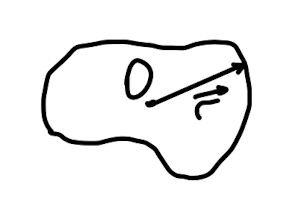
\includegraphics[width=\textwidth]{im/71.png} % Ваше изображение
\end{minipage}%
\hfill
\begin{minipage}[c]{0.55\textwidth} % Правая часть: текст
    \( \vec{H}=\vec{H_0}+(\vec{r}\gradd)\vec{H} \) 
\end{minipage}

\begin{gather*}
    \vec{F}=\frac{I}{c}\oint [d\vec{r}\times (\vec{r}\gradd)\vec{H}]=\frac{I}{c}\left[ \oint d\vec{r}(\vec{r}\gradd)\times \vec{H} \right]  \fbox{=}\\
    \oint d\vec{r}(\vec{r}\gradd)=\vec{r} \cancelto{0}{(\vec{r}\gradd)}| - \oint \vec{r}(d\vec{r}\gradd)=\frac{1}{2} \left[ d\vec{r}(\gradd\vec{r})-\vec{r}(d\vec{r}\gradd) \right]= \\
    =\frac{1}{2}\oint [\gradd \times [d\vec{r}\times \vec{r}]]  \\
    \text{Тогда:} \frac{I}{c}\oint d\vec{r}(\vec{r}\gradd)=\frac{I}{2c}\oint [[\vec{r}\times d\vec{r}]\times \gradd]=[\vec{m}\times \grad]  \\ 
    \fbox{=}[[\vec{m}\times \grad]\times \vec{H}]=[\overset{\downarrow}{\vec{H}}\times [\grad \times \vec{m}]]= \grad(\vec{H}\vec{m})-\vec{m}\cancelto{0}{\grad\vec{H}}
\end{gather*}

\[
\boxed{\vec{F}=\grad(\vec{H}\vec{m})}
\]
